\vspace{-0.5em}
\section{Economic Data Processing Inequality}
\vspace{-0.5em}
\label{sec:cracks}


Machine learning at its core is a data processing chain. 
While technical signal is carefully refined along this chain, economic equity is routinely removed from the original data generators---a circumstance we call \emph{economic data processing inequality}.  In our analysis
we identify three structural mechanisms convolving into this processing inequality: \emph{invisible provenance}, \emph{asymmetric bargaining power}, and \emph{inefficient price discovery}.  
These are not just concerns of economic welfare. As foundation models become economic actors or agents in their own right and data becomes a primary asset in that system of value creation, the link between data generation and weight harvesting that sustains today's learning algorithm is under strain.  Capital concentration and market inefficiency compound with each generation of data derivative, threatening to disenfranchise data generators. Data aggregators enjoy particularly powerful bargaining position at this time. This also raises the question whether data transformers, the actors refining data into model weights or labels,
and model monetizers are getting the best deal compared to an open market. \Cref{fig:deal-volume-figure} puts the scale and distribution of value in crass contrast: of the \$677.3m in reported revenue, creator royalties round to almost zero. Symptomatically, 57 of the 73 found deals do not disclose any revenue publicly. The problem of dark figures appears widespread on both the number of deals transacted and their revenue volumes. A healthier market must work for model monetizers, data aggregators, and data generators alike.

\vspace{1em}

\begin{wrapfigure}{l}{0.40\textwidth}
    \vspace{-0.6em}
    \centering
    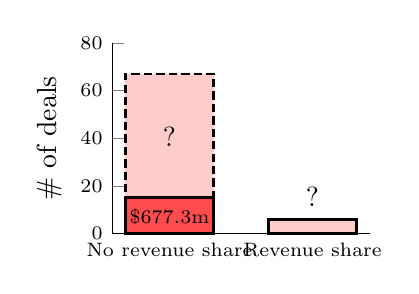
\begin{tikzpicture}
     \begin{axis}[
        axis lines*=left,
        ybar stacked,
        bar width=32pt,
        width=0.40\textwidth,
        height=4cm,
        ymin=0,
        ymax=80,
        ylabel={\# of deals},
        xtick=data,
        xtick style={draw=none},
        xticklabel style={font=\scriptsize},
        symbolic x coords={No revenue share,Revenue share},
        enlarge x limits=0.40,
        y tick label style={font=\scriptsize},
        ytick distance=20,
        clip=false,
        axis on top=true,
        z buffer=sort,
        after end axis/.code={%
          \node[font=\scriptsize, text=black, inner sep=1pt] at (axis cs:{No revenue share},7) {$\$677.3\mathrm{m}$};
          \node[font=\normalsize, text=black, inner sep=1pt] at (axis cs:{No revenue share},40.5) {?};
          \node[font=\normalsize, text=black, inner sep=1pt] at (axis cs:{Revenue share},15.5) {?};
        }
     ]
       \addplot+[draw=black, line width=1pt, fill=red!70]
         coordinates {
           (No revenue share,15)
           (Revenue share,0)
         };
       \addplot+[draw=black, dashed, dash pattern=on 3pt off 1.5pt, line width=1pt, fill=red!20]
         coordinates {
           (No revenue share,52)
           (Revenue share,0)
         };
        \addplot+[draw=black, line width=1pt, fill=red!20]
         coordinates {
           (No revenue share,0)
           (Revenue share,6)
         };

     \end{axis}
    \end{tikzpicture}
    \vspace{-0.6em}
    \caption{Counts of data deals with and without revenue share information. Left bar (No revenue share): solid segment (15 deals) corresponds to deals where public sources quoted a revenue volume. If ranges are given we conservatively take the floor of that range. Total sum of disclosed revenue volume is \$677.3m. The dashed segment (52 deals) indicates additional deals without revenue share and shows the problem of dark figures in this space. Right bar (Revenue share): 6 deals feature some revenue sharing information to generators, only one has public information on revenue (\$2.5k).}
    \vspace{-0.5em}
    \label{fig:deal-volume-figure}
  \end{wrapfigure}
 

\textbf{Invisible Provenance.} Once data is copied beyond its point of creation, contextual metadata—license, collection method, consent—often gets lost \cite{longpre2024large}. 
Provenance failures are by no means confined to academic benchmarks: they surface in healthcare (\cite{deepmindnhs2017}), social media (\cite{pinterest2025}), or open-source code (\cite{githubcopilotlawsuit2022}). As early as 2017, we have cases like the DeepMind--Royal Free breach where the UK Information Commissioner ruled that data generators ``were not adequately informed that their data would be used'' in deep learning products \cite{icouk2017}.
These types of disconnects between data's underlying license and its actual appeat to be a structural problem across the board and concerns many community datasets at large. An analysis on more than 1800 datasets has shown that more than 70\% have license omissions and datasets with licenses have error rates of over 50\% \cite{longpre2024large}.
This causes provenance loss for data generators and legal uncertainty for data transformers and model monetizers. And the implications of this license uncertainty affect the value chain not only during training but also during inference on model weights. Across modalities, models can be shown to regurgitate images \cite{carlini2023extracting} and text \cite{scihub2025} including content the model provider may not have the license for. In publicly disclosed license deals, the provenance disconnect between data and value generation already shows: a negligable fraction make provisions for revenue sharing with data generators (\Cref{app:data-deals-full-table} and \Cref{tab:data-deals-joint}).
Provenance gaps cascade through the value chain.  The problem compounds once models are fine-tuned on material they themselves have produced \cite{shumailov2024ai,gerstgrasser2024is}.
Already models train on a mix of original human content and synthetic content, which creates increasingly complex lineage graphs.
Without robust, practical provenance a downstream user cannot audit permissions, enforce attribution, or route royalties, which in turn can chill secondary innovation and disrupt the feedback loop that rewards originators.



\begin{wraptable}{r}{0.40\textwidth}
\vspace{-1em}
    \scriptsize
    \centering
    \begin{tabular}{l l l}
        \toprule
        & \textbf{Category} & \textbf{Deals} \\
        \midrule
        \multirow{4}{*}{\textbf{Top Types}} & News  & 26 \\
                                   & Images     & 16\\
                                   & Academic & 15 \\
                                   & UGC      & 14\\
        \midrule
        \multirow{4}{*}{\textbf{Top Buyers}} & OpenAI & 24\\
                                         & Undisclosed & 8\\
                                         & Google & 6 \\
                                         & Perplexity & 3 \\
        \midrule
        \multirow{5}{*}{\textbf{Payment}} & Amount disclosed & 16 \\
                                            & Undisclosed & 57 \\
                                           & Recurring & 3 \\
                                           & Generator split & 6 \\
                                           & Litigation & 4 \\
        \bottomrule
    \end{tabular}
    \caption{Aggregated snapshot on types, buyers and payment of 73 publicly disclosed data deals from \Cref{tab:data-deals-joint}.}
    \vspace{-0.5em}
    \label{tab:deal-summary-filled}
\end{wraptable} 


\textbf{Asymmetric Bargaining Power.} Even when provenance is intact, individual data generators are typically left out of deals between aggregators and model monetizers. Community platforms such as Reddit (\$60~million per annum from Google~\cite{googlereddit2024}), Stack Overflow (bundled into Gemini~\cite{googlestackoverflow2024}), and stock libraries like Shutterstock (multiple eight-figure licences in 2023–2024) all negotiate encompassing deals while offering creators click-wrap terms that grant sweeping reuse rights. Despite monitoring agencies such as the US Federal Trade Commission warning companies that such practices may be deemed deceptive \cite{ftc2024}, many platforms that host user-generated content (UGC) such as Google, Adobe, Snap, X or Meta have been modifying their terms of service regardless \cite{nyt2024tech}.
This power asymmetry also comes to bear in publicly disclosed data deals. More than 40\% of known transactions were conducted by OpenAI/Microsoft, Google, or Perplexity on the buying side (\Cref{tab:deal-summary-filled}), while aggregators bundle the receipts. These imbalances can snowball.  Low marginal inference cost and winner-takes-most network effects channel control surplus to a handful of aggregators and monetizers. Maybe unintuitively this asymmetry also has the potential to harm the model monetizers who buy the data, because they negotiate with aggregator platforms rather than the generators directly in an open market.
Rosen's "superstar" economics \cite{rosen1981economics} suggests—and recent market caps of large AI companies confirm—that the top few firms stand to capture a lion's share of AI rents.  
Of the 73 transactions in \Cref{app:data-deals-full-table} only six mention any revenue-share with contributors.  In contrast, several deals, marked "L", are under litigation, signalling that they were hedged under the prospect of court action rather than negotiated at arm's length.

\textbf{Inefficient Price Discovery.} Where money does change hands it is almost always a lump-sum buy-out.  News media licenses are illustrative: Associated Press agreed a two-year, flat-fee deal (amount undisclosed)~\cite{openaiap2023}; News Corp settled for roughly \$250~million across five years~\cite{openainewscorp2024}; Axel Springer and Dotdash Meredith followed the same template.  To the extent of public disclosure, these contracts do not appear to include royalty escalators for generators tied to usage, retraining, or downstream revenue.  
All of this plays out against a shifting legal backdrop: ongoing cases such as \emph{Getty Images v.~Stability AI}, \emph{NYT v.~OpenAI}, and \emph{News/Media Alliance v.~Cohere} hint that copyright doctrine, usage rights, and privacy statutes have yet to converge on generative training. Until clarity emerges, originators must choose between costly litigation and acquiescing to not participate in the market. In this sense, static payments are reinforced by the provenance gap.  Once an originator has been taken out of the market equation, they have no financial stake anymore to participate in data quality, maintainenance of consent records, or police misuse, while the buyer internalizes much of the upside of any future innovation.

\noindent These three faults interact multiplicatively: missing provenance, undercuts bargaining, weak bargaining yields one-shot buy-outs, and buy-outs remove any incentive to invest in provenance.  Breaking the cycle and creating an open market that maximizes overall welfare therefore requires technical and institutional interventions that address \emph{all three dimensions at once}. 
